\chapter{Metodología y Diseño del Sistema}\label{cap:metodologia}
Este capítulo describe cómo se construyó el sistema y por qué se tomaron las principales decisiones de diseño. Se presenta primero el enfoque metodológico y las fases de desarrollo; luego, la arquitectura modular de la biblioteca y el flujo de una iteración de entrenamiento; después, la estrategia de verificación y de reproducibilidad; y, por último, el diseño de los tres experimentos.

\section{Enfoque metodológico}
El proyecto adopta un enfoque cuantitativo de tipo experimental aplicado \citep{hernandez2018}: se construye un artefacto de software, se formulan hipótesis verificables sobre su comportamiento ---por ejemplo, que una red sin capa oculta no puede resolver XOR y que una red 2-4-1 sí puede--- y se contrastan mediante ejecuciones reproducibles cuyos resultados se registran automáticamente. El desarrollo del software sigue un modelo incremental guiado por pruebas: cada módulo se implementa junto con sus pruebas unitarias y no se avanza a la fase siguiente hasta que todas las pruebas de la fase actual se aprueban. Este criterio de avance convierte cada fase en un entregable verificable y evita que los errores de las capas inferiores ---por ejemplo, un índice mal calculado en la multiplicación matricial--- se propaguen y se manifiesten como fallos difíciles de diagnosticar en el entrenamiento.

\section{Fases de desarrollo}
La Figura~\ref{fig:fases} presenta las nueve fases del proyecto, agrupadas en cuatro etapas: fundamentos matemáticos (fases 1--4), aprendizaje (fases 5--6), experimentación (fases 7--8) y difusión (fase 9). Cada fase indica su entregable principal y la verificación que habilita el paso a la fase siguiente.

\begin{figure}[!htbp]
\caption{Fases de la metodología incremental del proyecto}\label{fig:fases}
\centering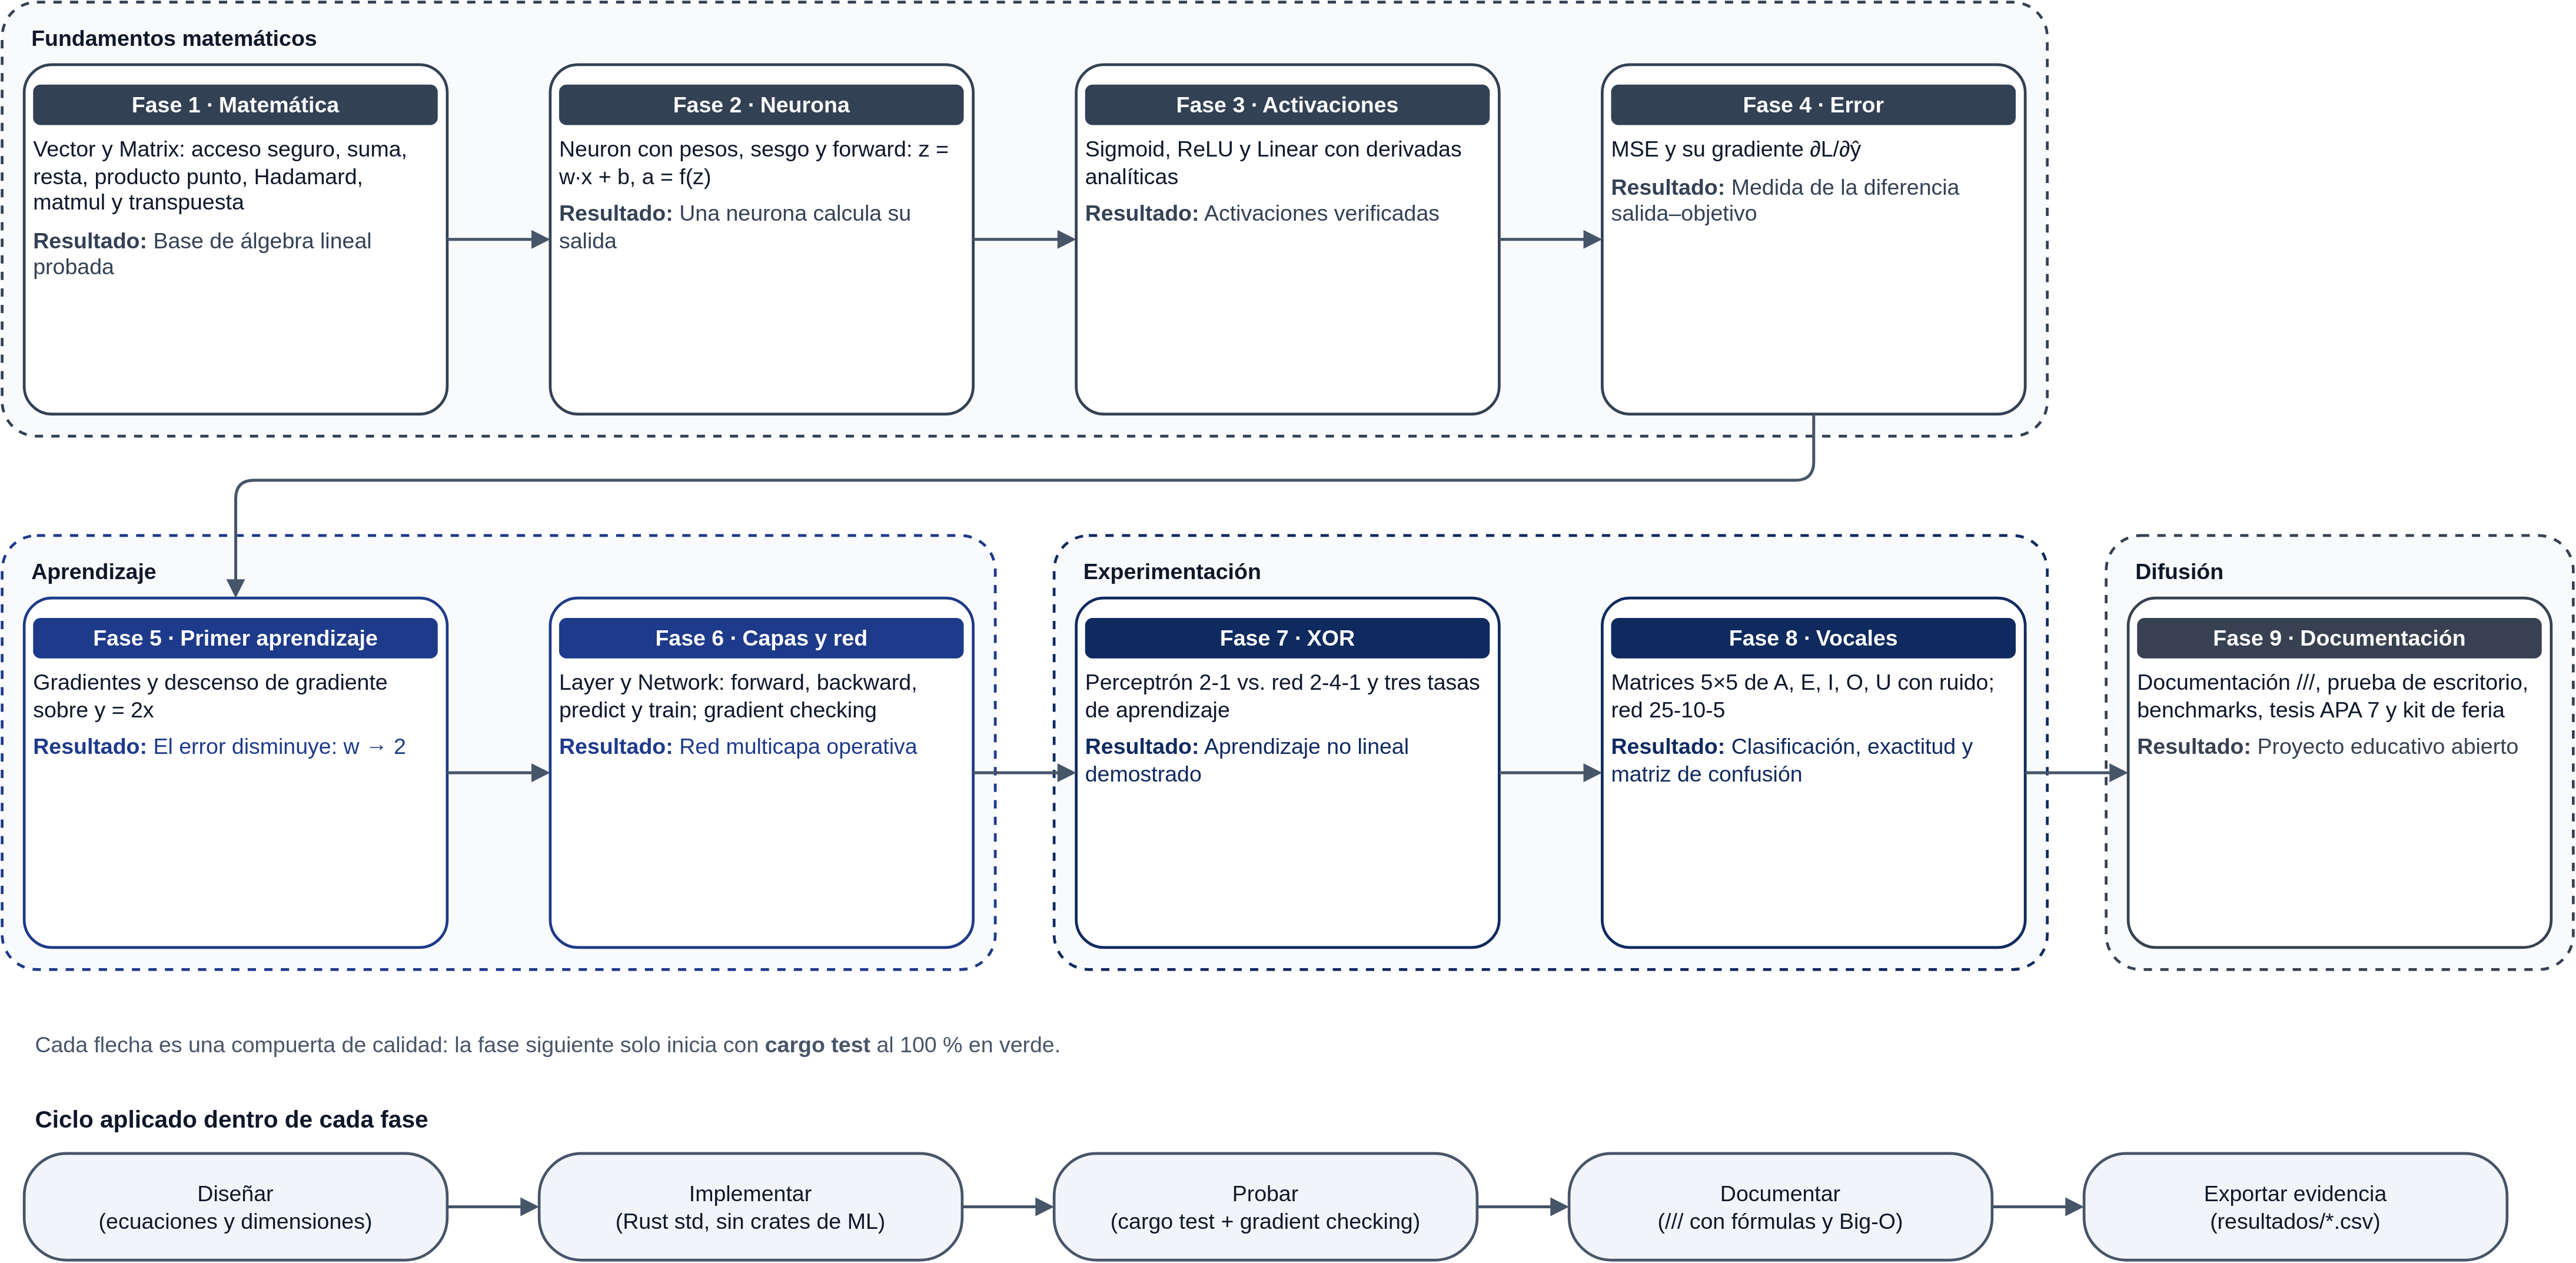
\includegraphics[width=\textwidth,height=0.5\textheight,keepaspectratio]{figuras/diag05_fases_metodologia.png}
\fuente{Cada fase concluye con la aprobación de sus pruebas unitarias. Diagrama editable: \texttt{diagramas/05\_fases\_metodologia.drawio}.}
\end{figure}

La Tabla~\ref{tab:fases} detalla las fases en forma tabular, junto con los módulos de código que producen y las pruebas que las validan.

\begin{table}[!htbp]
\caption{Fases de desarrollo, entregables y criterios de aceptación}\label{tab:fases}
\small
\begin{tabularx}{\textwidth}{@{}l >{\raggedright}p{3.4cm} >{\raggedright}X >{\raggedright\arraybackslash}p{3.6cm}@{}}
\toprule
Fase & Nombre & Entregable & Criterio de aceptación \\
\midrule
1 & Matemática & \texttt{Vector}, \texttt{Matrix}, \texttt{MathError}, \texttt{Rng} & 15 pruebas de \texttt{math} \\
2 & Neurona & \texttt{Neuron}: $z=\mathbf{w}\cdot\mathbf{x}+b$, $a=f(z)$ & Cálculo manual reproducido \\
3 & Activaciones & Sigmoid, ReLU y lineal con sus derivadas & Derivadas verificadas numéricamente \\
4 & Error & \texttt{Mse} y su gradiente $\partial L/\partial\hat{y}$ & Valores conocidos y \emph{gradient checking} \\
5 & Primer aprendizaje & Descenso de gradiente sobre $y=2x$ & El MSE disminuye y $w\to 2$ \\
6 & Capas y red & \texttt{Layer} y \texttt{Network}: \texttt{forward}, \texttt{backward}, \texttt{predict}, \texttt{train} & \emph{Gradient checking} de la red \\
7 & XOR & Perceptrón 2-1 frente a red 2-4-1 y tres tasas de aprendizaje & Aprendizaje no lineal demostrado \\
8 & Vocales & Red 25-10-5 sobre matrices $5\times5$ con ruido & Exactitud y matriz de confusión en CSV \\
9 & Documentación & Prueba de escritorio, \emph{benchmarks}, tesis, diagramas y material de feria & PDF y DOCX sin referencias rotas \\
\bottomrule
\end{tabularx}
\fuente{Elaboración propia. El número de pruebas por módulo se detalla en la Tabla~\ref{tab:pruebas}.}
\end{table}

\section{Requisitos del sistema}
Antes de diseñar la arquitectura se establecieron los requisitos funcionales y no funcionales que el motor debía cumplir. Los requisitos funcionales comprenden: representar vectores y matrices con sus operaciones; construir redes de topología arbitraria a partir de una lista de tamaños de capa y de funciones de activación; propagar una entrada hacia adelante; calcular el gradiente de la pérdida mediante retropropagación; actualizar los parámetros por descenso de gradiente; ejecutar los tres experimentos y la prueba de escritorio; medir tiempos; y exportar todos los resultados en formato CSV. Los requisitos no funcionales comprenden: no utilizar dependencias externas; garantizar la reproducibilidad exacta mediante una semilla; detectar los errores de dimensión sin interrumpir abruptamente el programa; documentar cada elemento público con comentarios \texttt{///}; y superar el análisis estático de \texttt{cargo clippy} sin advertencias.

\section{Arquitectura modular}
El código se organiza como una biblioteca (\texttt{src/lib.rs}) y un binario de línea de comandos (\texttt{src/main.rs}). La biblioteca se divide en tres módulos con responsabilidades separadas y dependencias en un solo sentido: \texttt{experiments} depende de \texttt{nn}, y \texttt{nn} depende de \texttt{math}, pero nunca a la inversa. La Figura~\ref{fig:arquitectura} representa esta organización.

\begin{figure}[!htbp]
\caption{Arquitectura modular del motor en Rust}\label{fig:arquitectura}
\centering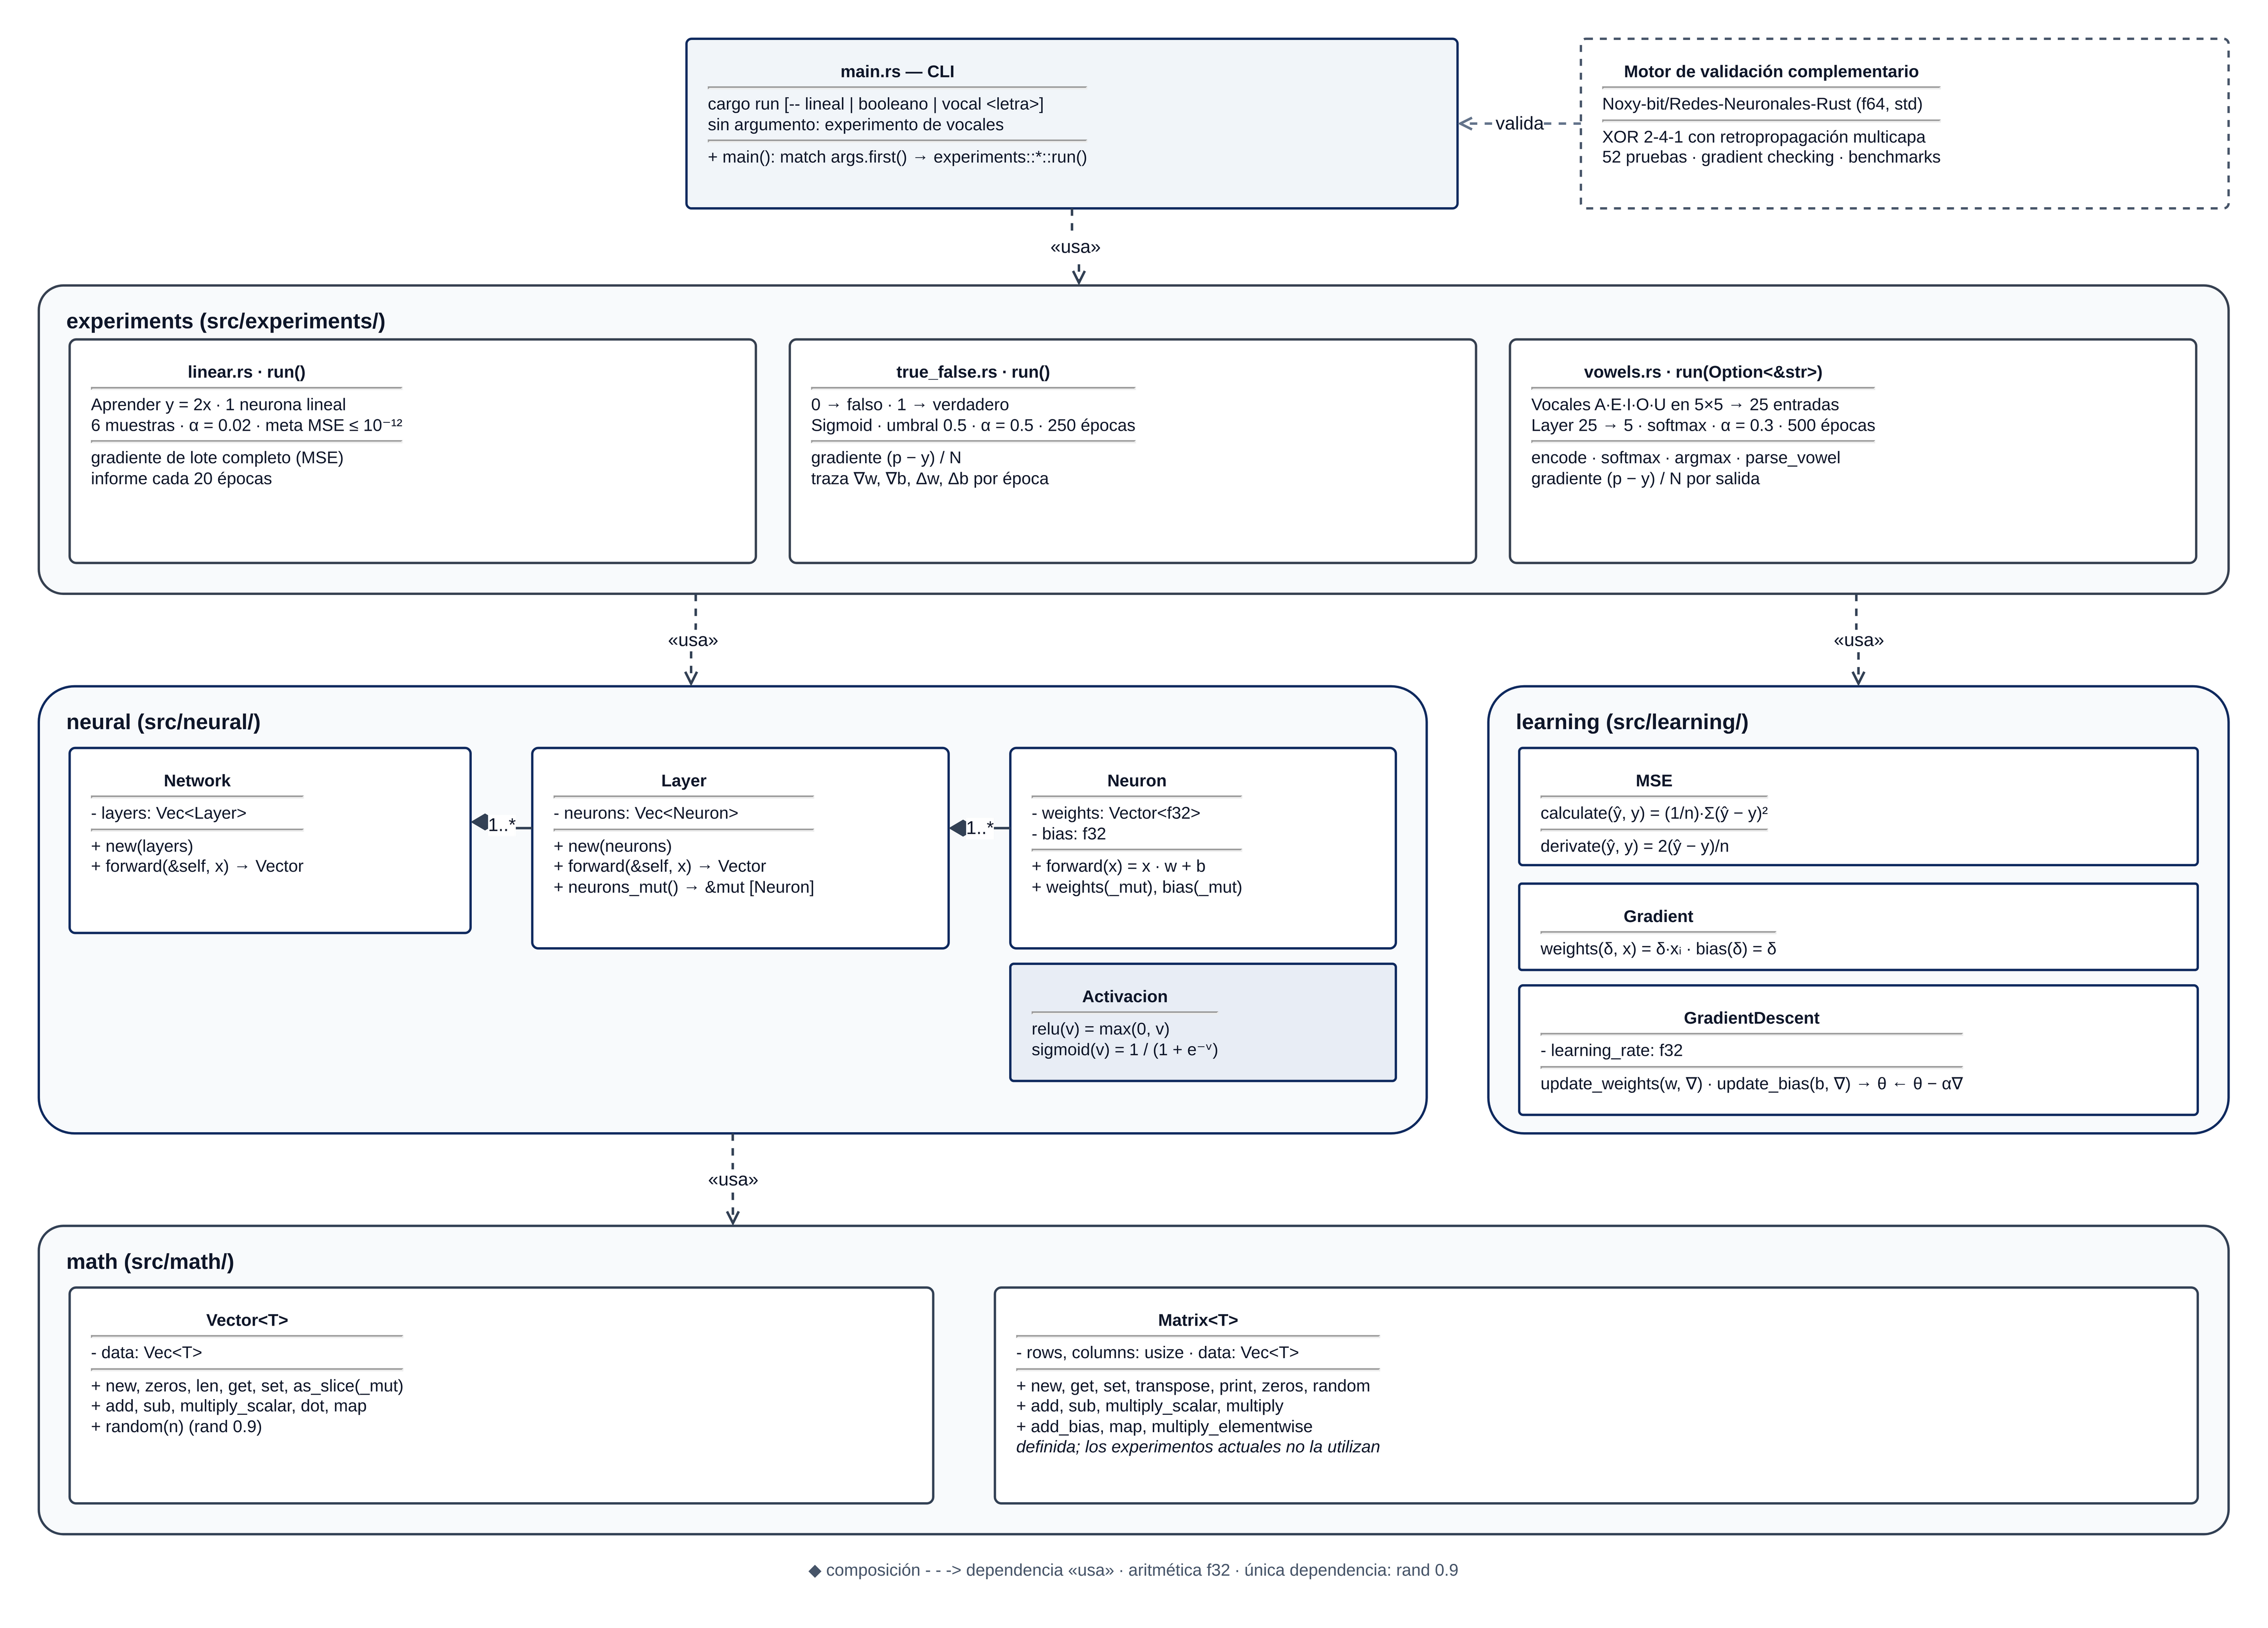
\includegraphics[width=\textwidth,height=0.55\textheight,keepaspectratio]{figuras/diag02_arquitectura_rust.png}
\fuente{Las flechas indican dependencias de uso entre módulos. Diagrama editable: \texttt{diagramas/02\_arquitectura\_modulos\_rust.drawio}.}
\end{figure}

La Tabla~\ref{tab:arquitectura} describe la responsabilidad de cada archivo. La separación permite probar cada componente de forma aislada y sustituirlo sin afectar a los demás; por ejemplo, la estructura \texttt{Network} no conoce la fórmula de ninguna función de activación, sino que delega en el trait \texttt{ActivationFn}.

\begin{table}[!htbp]
\caption{Módulos de la arquitectura implementada}\label{tab:arquitectura}
\small
\begin{tabularx}{\textwidth}{@{}l >{\raggedright\arraybackslash}X@{}}
\toprule
Archivo & Responsabilidad \\
\midrule
\texttt{math/vector.rs} & Vector $\mathbb{R}^n$: suma, resta, producto punto, Hadamard, escalamiento, norma, \texttt{argmax}. \\
\texttt{math/matrix.rs} & Matriz $\mathbb{R}^{m\times n}$ \emph{row-major}: producto matricial, matriz-vector, transpuesta, producto exterior. \\
\texttt{math/error.rs} & Tipo \texttt{MathError} para dimensiones incompatibles, índices fuera de rango y argumentos inválidos. \\
\texttt{math/rng.rs} & Generador pseudoaleatorio SplitMix64 reproducible y barajado Fisher--Yates. \\
\texttt{nn/activation.rs} & Trait \texttt{ActivationFn}; Sigmoid, ReLU y lineal con derivadas analíticas. \\
\texttt{nn/loss.rs} & Trait \texttt{LossFn}; MSE y su gradiente. \\
\texttt{nn/neuron.rs} & Neurona individual: pesos, sesgo, suma ponderada y activación. \\
\texttt{nn/layer.rs} & Capa densa: \texttt{forward}, \texttt{backward}, gradientes y actualización. \\
\texttt{nn/network.rs} & Red multicapa: \texttt{forward}, \texttt{backward}, \texttt{predict}, \texttt{train}, evaluación. \\
\texttt{experiments/} & Tres experimentos, prueba de escritorio, \emph{benchmarks} y escritura de CSV. \\
\texttt{main.rs} & CLI reproducible: \texttt{--all}, \texttt{--exp1..3}, \texttt{--escritorio}, \texttt{--bench}, \texttt{--export}, \texttt{--seed}. \\
\bottomrule
\end{tabularx}
\fuente{El archivo \texttt{Cargo.toml} no declara ninguna dependencia: todo el sistema utiliza exclusivamente la biblioteca estándar de Rust.}
\end{table}

\section{Decisiones de diseño}
Varias decisiones de diseño condicionan el comportamiento del sistema y merecen justificarse explícitamente.

\subsection{Almacenamiento contiguo por filas}
Se eligió almacenar cada matriz en un único \texttt{Vec<f64>} en lugar de un vector de vectores. Esta representación reduce el número de reservas de memoria, mejora la localidad de referencia en el producto matriz-vector ---que recorre cada fila de forma secuencial--- y simplifica la validación de dimensiones, pues basta comprobar que la longitud del arreglo sea $m\cdot n$.

\subsection{Errores como valores}
Todas las operaciones susceptibles de fallar devuelven \texttt{Result}. La alternativa ---provocar un pánico ante dimensiones incompatibles--- habría sido más breve, pero habría impedido probar los casos de error y habría convertido un descuido de configuración en una terminación abrupta del programa. Las pruebas \texttt{errores\_de\_dimension}, \texttt{mse\_errores\_de\_dimension} y \texttt{backward\_sin\_forward\_es\_error} verifican precisamente estos caminos.

\subsection{Caché de valores intermedios en la capa}
Cada capa guarda la última entrada recibida, el vector $\mathbf{z}$, la salida, el vector $\boldsymbol{\delta}$ y los gradientes. Esta decisión, que cuesta memoria proporcional al tamaño de la capa, evita recalcular la propagación hacia adelante durante la retropropagación y permite que la prueba de escritorio lea directamente los valores intermedios de cada neurona. Para la inferencia se ofrece además el método \texttt{predict}, que recibe la red por referencia inmutable y no modifica la caché.

\subsection{Generador pseudoaleatorio propio}
La biblioteca estándar de Rust no incluye un generador de números aleatorios con semilla. En lugar de añadir una dependencia, se implementó SplitMix64, un generador de 64 bits con buena calidad estadística para inicialización y muestreo, cuya secuencia de referencia se verifica en la prueba \texttt{vector\_de\_referencia\_splitmix64}. La semilla por defecto es 42 y puede modificarse con el argumento \texttt{--seed}.

\subsection{Activaciones mediante trait y enumeración}
Las funciones de activación implementan el trait \texttt{ActivationFn}, y la enumeración \texttt{Activation} despacha a cada implementación mediante \texttt{match}. Esta combinación permite guardar la activación de cada capa como un valor pequeño y copiable, compararla y exportarla por nombre, mientras que el trait conserva la posibilidad de extender el sistema con nuevas funciones.

\section{Flujo de entrenamiento}
La Figura~\ref{fig:flujo} representa el algoritmo de entrenamiento implementado. Una iteración consta de cuatro pasos: (1) la entrada $\mathbf{x}$ atraviesa cada capa calculando $\mathbf{z}^{(l)}$ y $\mathbf{a}^{(l)}$, que se almacenan en caché; (2) se calcula la pérdida MSE y su gradiente respecto a la salida; (3) cada capa, de la última a la primera, calcula $\boldsymbol{\delta}^{(l)}$, sus gradientes y el gradiente que transmite a la capa anterior; y (4) todos los parámetros se actualizan con la Ecuación~\eqref{eq:gd}. Al terminar cada época se evalúa el MSE sobre el conjunto completo y se registra en el archivo CSV del experimento.

\begin{figure}[!htbp]
\caption{Diagrama de flujo del entrenamiento con propagación hacia adelante y retropropagación}\label{fig:flujo}
\centering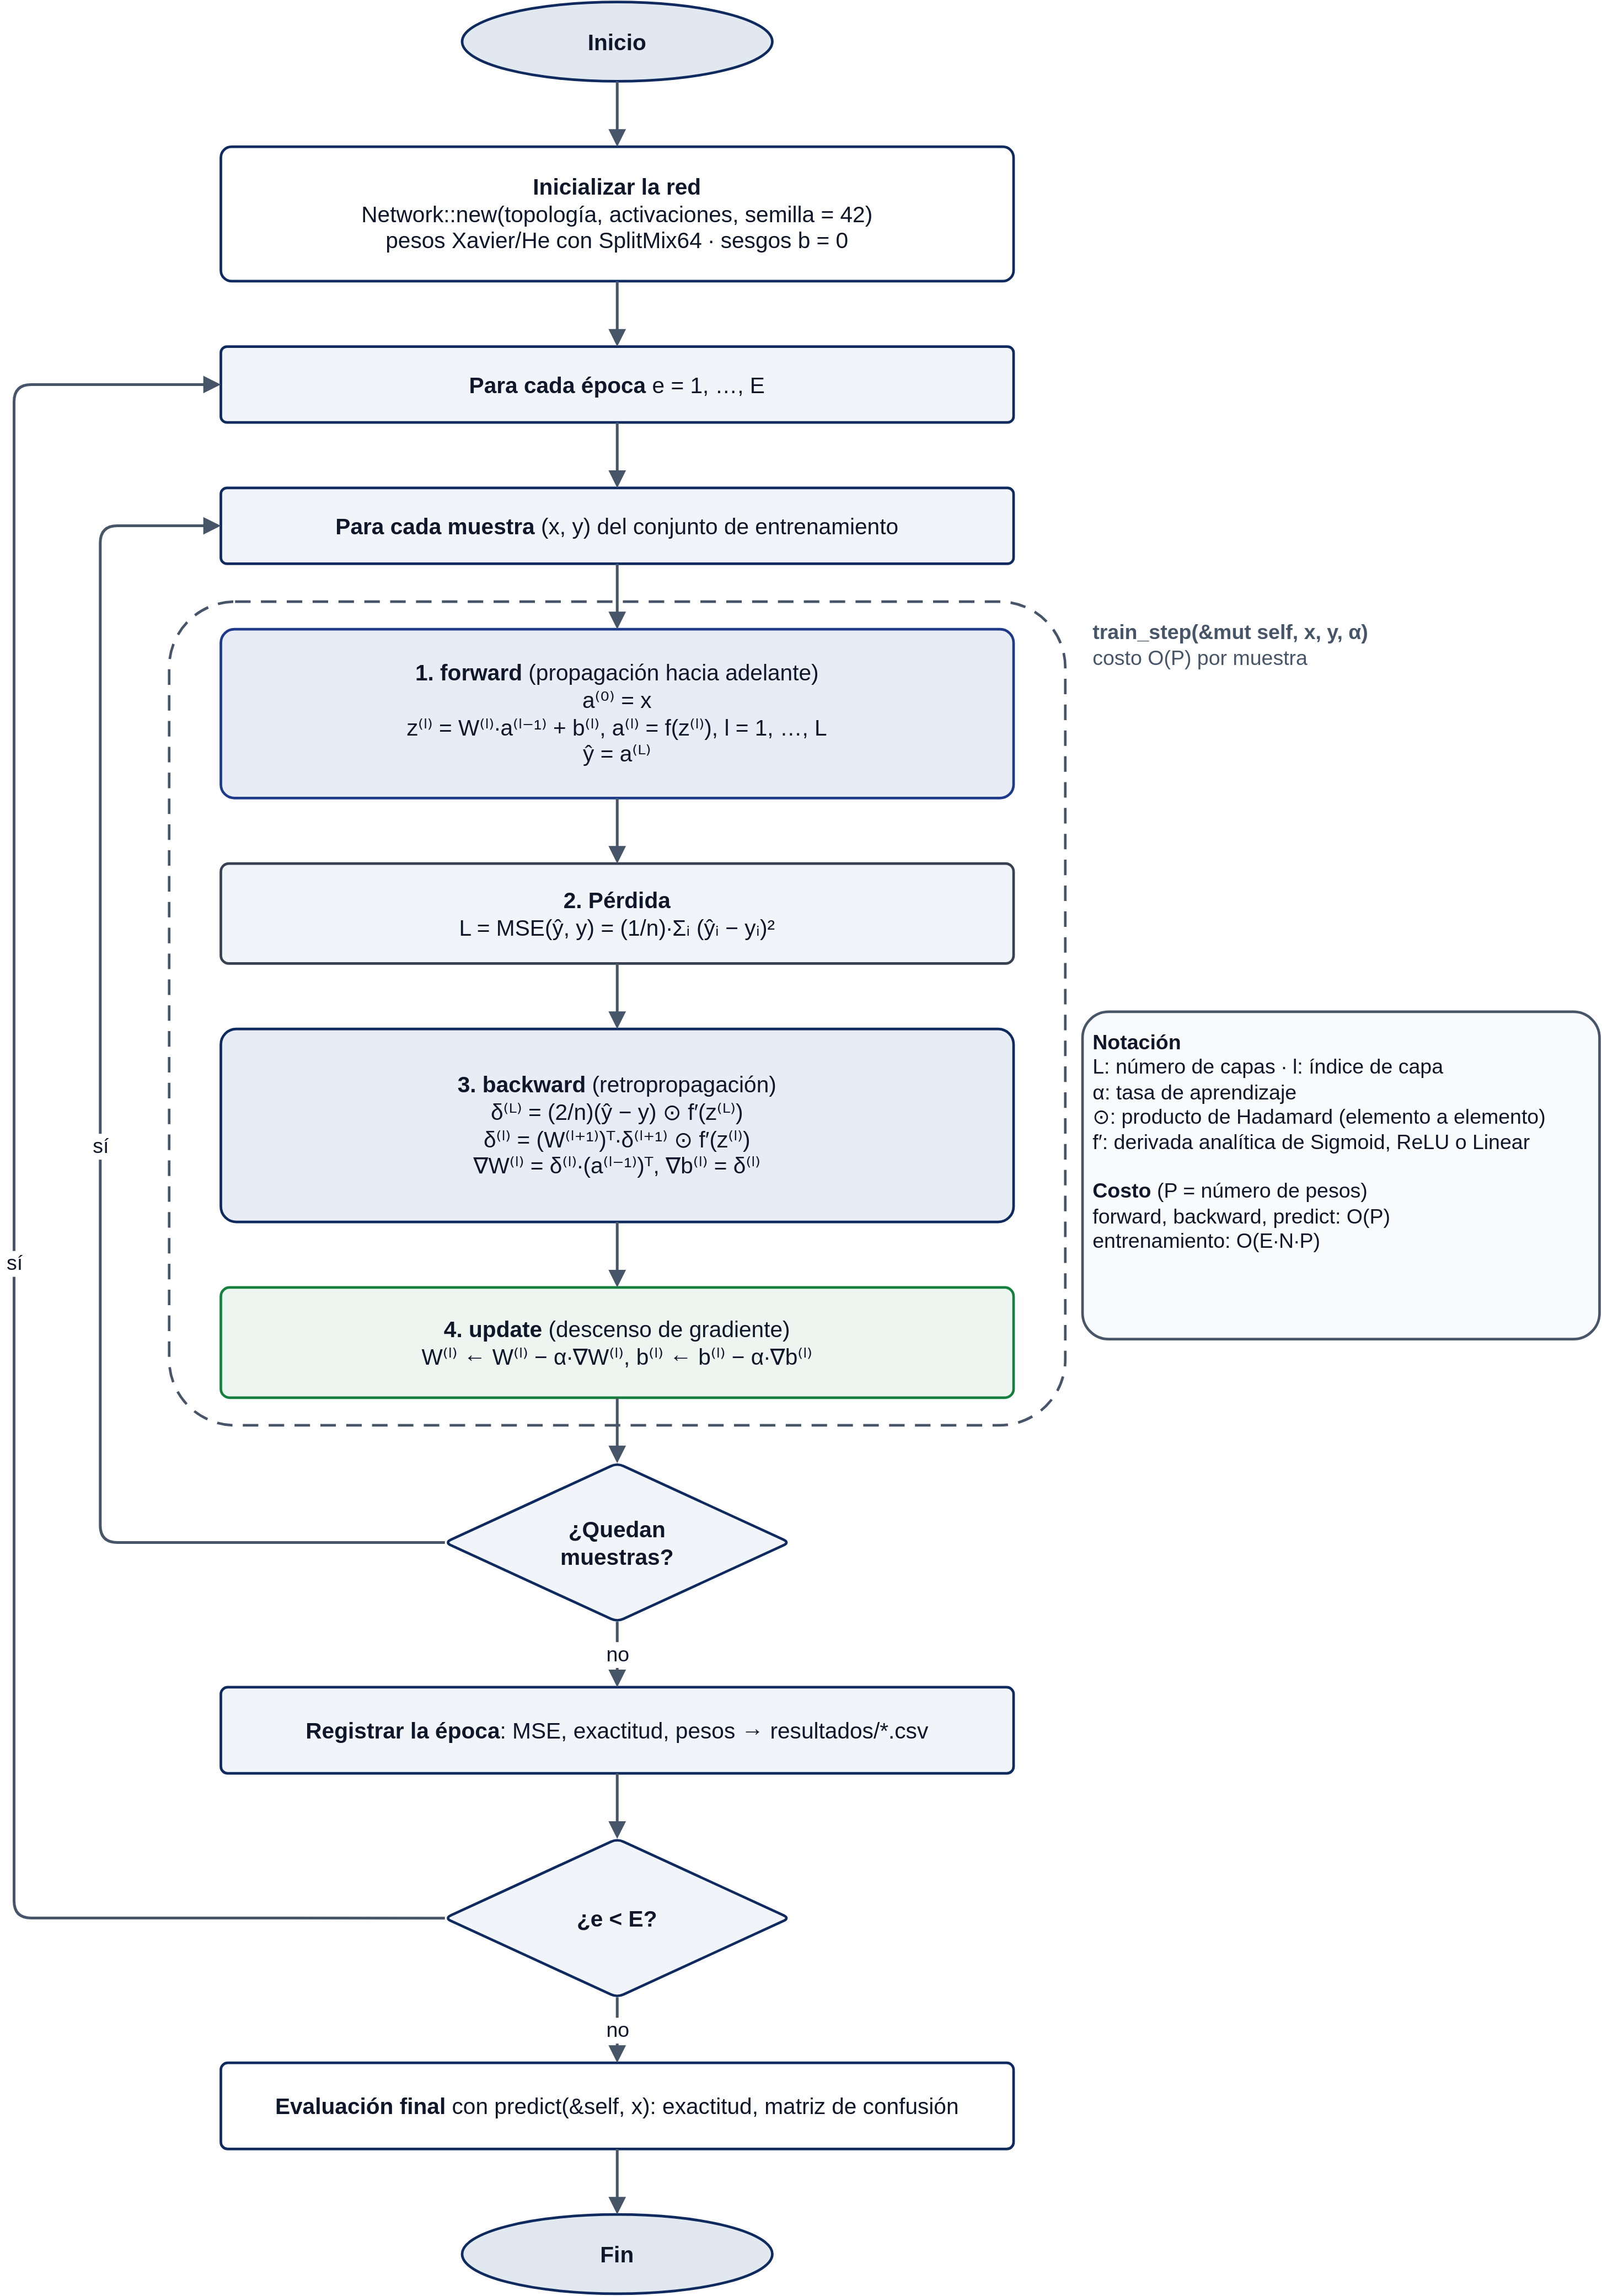
\includegraphics[width=\textwidth,height=0.72\textheight,keepaspectratio]{figuras/diag03_flujo_entrenamiento.png}
\fuente{El ciclo interno recorre las muestras y el externo las épocas. Diagrama editable: \texttt{diagramas/03\_flujo\_forward\_backprop.drawio}.}
\end{figure}

\section{Estrategia de verificación}
La verificación combina cuatro tipos de pruebas automatizadas. Las pruebas de valores conocidos comparan la salida de una función con un resultado calculado a mano, por ejemplo $\sigma(0) = 0.5$ o la salida de una capa con pesos fijos. Las pruebas de errores comprueban que las operaciones con dimensiones incompatibles devuelvan el error esperado. Las pruebas de propiedades verifican identidades matemáticas y de determinismo, como que la misma semilla produzca la misma secuencia o que el barajado sea una permutación. Finalmente, las pruebas de integración entrenan redes reales y verifican su convergencia y la corrección numérica de sus gradientes. La Tabla~\ref{tab:pruebas} presenta la distribución de las 52 pruebas por módulo.

\begin{table}[!htbp]
\caption{Distribución de las pruebas automatizadas por módulo}\label{tab:pruebas}
\small
\begin{tabularx}{\textwidth}{@{}l r >{\raggedright\arraybackslash}X@{}}
\toprule
Módulo & Pruebas & Aspectos verificados \\
\midrule
\texttt{math::vector} & 4 & Creación, acceso seguro, operaciones, \texttt{argmax}, errores de dimensión \\
\texttt{math::matrix} & 6 & Acceso, operaciones elemento a elemento, producto matricial, transpuesta, producto exterior \\
\texttt{math::rng} & 4 & Secuencia de referencia, determinismo, rangos uniformes, permutación \\
\texttt{math::error} & 1 & Mensajes descriptivos \\
\texttt{nn::activation} & 4 & Valores conocidos, despacho, derivadas por \emph{gradient checking} \\
\texttt{nn::loss} & 3 & Valores conocidos, errores, \emph{gradient checking} \\
\texttt{nn::neuron} & 3 & Cálculo manual, errores, inicialización reproducible \\
\texttt{nn::layer} & 4 & Dimensiones, cálculo manual, retropropagación y actualización \\
\texttt{nn::network} & 11 & Validaciones, \emph{gradient checking} (2-4-1, 3-5-4-2, 25-10-5), convergencia \\
\texttt{experiments} & 11 & CSV, exactitud, experimentos 1--3, prueba de escritorio, \emph{benchmarks} \\
\texttt{main} (CLI) & 1 & Interpretación de argumentos y errores \\
\midrule
Total & 52 & 51 pruebas de biblioteca y 1 de binario \\
\bottomrule
\end{tabularx}
\fuente{Conteo obtenido de la salida real de \texttt{cargo test} (Anexo~\ref{anx:tests}).}
\end{table}

\section{Reproducibilidad}
Para que cualquier evaluador obtenga exactamente los mismos resultados, se tomaron tres medidas. Primero, todos los pesos iniciales, el orden aleatorio y el ruido de los datos se generan con el PRNG propio a partir de una semilla fija, de modo que la misma semilla produce los mismos números en cualquier equipo. Segundo, los conjuntos de datos se definen explícitamente en el código fuente y no dependen de archivos externos. Tercero, el binario escribe todos los resultados en archivos CSV, y las tablas, cifras y gráficas de este documento se generan exclusivamente a partir de esos archivos mediante los scripts \path{tesis/scripts/resultados.py} y \path{scripts/generar_graficas.py}. La presentación de tablas, figuras, citas y referencias sigue el manual de publicaciones de la American Psychological Association en su séptima edición \citep{apa2020}. Los tiempos de ejecución son la única magnitud que depende del equipo; por ello se informan junto con el sistema operativo, la arquitectura y el perfil de compilación.

\section{Diseño de los experimentos}
Los tres experimentos se diseñaron con complejidad creciente, de modo que cada uno valide una capacidad adicional del motor. La Tabla~\ref{tab:diseno-exp} resume su configuración.

\begin{table}[!htbp]
\caption{Configuración de los experimentos}\label{tab:diseno-exp}
\footnotesize
\begin{tabularx}{\textwidth}{@{}l >{\raggedright}X >{\raggedright}X >{\raggedright\arraybackslash}X@{}}
\toprule
Aspecto & Experimento 1 & Experimento 2 & Experimento 3 \\
\midrule
Problema & Regresión $y=2x$ & Compuerta XOR & Vocales A, E, I, O, U \\
Capacidad validada & Ajuste lineal & Separación no lineal & Clasificación multiclase con ruido \\
Arquitectura & 1-1 (lineal) & 2-1 y 2-4-1 (Sigmoid) & 25-10-5 (Sigmoid) \\
Parámetros & 2 & 3 y 17 & 315 \\
Épocas & \EunoEpocas & \EdosEpocas & \EtresEpocas \\
Tasa $\alpha$ & \EunoAlpha & \EdosAlpha{} (y 0.01, 50) & \EtresAlpha \\
Datos & 5 pares $(x, 2x)$ & 4 combinaciones binarias & \EtresNEnt{} de entrenamiento, \EtresNPru{} de prueba \\
Métricas & MSE, $w$, $b$, predicción & MSE, exactitud, frontera & MSE, exactitud, confusión \\
\bottomrule
\end{tabularx}
\fuente{Valores leídos de \path{resultados/resumen.csv}. Todas las ejecuciones usan semilla 42.}
\end{table}

El Experimento~1 tiene solución analítica conocida ($w=2$, $b=0$), por lo que permite verificar cuantitativamente la convergencia. El Experimento~2 reproduce el argumento histórico de \citet{minsky1969} y su superación mediante una capa oculta, y añade un estudio del efecto de la tasa de aprendizaje. El Experimento~3 introduce un problema multiclase con 25 entradas, separa estrictamente los conjuntos de entrenamiento y de prueba y evalúa la robustez frente a niveles de ruido mayores que los vistos durante el entrenamiento.
